\documentclass{article}
% --- STANDARD PACKAGES ---
% \usepackage{PRIMEarxiv}
\usepackage{microtype}
\usepackage[utf8]{inputenc}
\usepackage[T1]{fontenc}
\usepackage{xurl}
\usepackage{url}
\usepackage{booktabs} % For professional tables
\usepackage{amsfonts}
\usepackage{nicefrac}
\usepackage{keyval}
\usepackage{fancyhdr}
\usepackage{graphicx}
\usepackage{amsmath}    % For advanced math environments
\usepackage{amssymb}    % For blackboard bold, etc.
\usepackage{tikz}
\usetikzlibrary{shapes.geometric, arrows.meta, positioning}
\usepackage[margin=1in]{geometry}       % Widen text area
\usepackage{setspace}                   % For line spacing control
\setstretch{1.1}                        % Slightly tighter than article default
\usepackage[compact]{titlesec}
\usepackage{hyperref}
\graphicspath{{media/}}


%Header
\pagestyle{fancy}
\thispagestyle{empty}
\rhead{\textit{ }} 

% Update your Headers here
\fancyhead[LO]{Unaware Adversaries: A Framework for Characterizing Emergent Conflict Between Non-Coordinating Agents}
% \fancyhead[RE]{Scott VanRavenswaay} % Firstauthor et al. if more than 2 - must use \documentclass[twoside]{article}

%% Title
\title{Unaware Adversaries: A Framework for Characterizing Emergent Conflict Between Non-Coordinating Agents}

\author{
  Scott VanRavenswaay \\
  \texttt{scottvr@gmail.com} \\
}

\begin{document}
\begin{center}
  \rule{\textwidth}{0.4pt}\vspace{1ex}

  {\LARGE Unaware Adversaries: A Framework for Characterizing Emergent Conflict Between Non-Coordinating Agents}

  \vspace{1ex}
  {\large Scott VanRavenswaay\\
  \texttt{scottvr@gmail.com}}\\
  \vspace{0.5ex}
  {\small February 2026}

  \vspace{1ex}
  \rule{\textwidth}{0.4pt}
\end{center}

\vspace{2ex}

\begin{abstract}
In many complex systems, constituent agents engage in adversarial behavior without explicit awareness or intent. These ``unaware adversaries'' operate based on localized objectives and feedback, yet their interactions within a shared environment result in mutual disruption, resource competition, or functional conflict. This paper formally defines this phenomenon and situates it within existing literature on systems theory. We present and analyze several case studies—including closed-loop, open-loop, and designed conflicts—to build a taxonomy of adversarial typologies. By demonstrating how this framework can be used as a generative tool for analysis and design, we derive illustrative mitigation strategies for problems in fields as diverse as generative modeling and internet routing. The result is a framework intended to help identify, classify, and resolve a pervasive yet under-examined class of system failures, and to generate potential new avenues for research by applying the framework beyond just mitigation.
\end{abstract}

\vspace{1ex}
\noindent\textbf{Keywords:} unaware adversaries, emergent conflict, system dynamics, feedback control loops, multi-agent systems, generative adversarial networks, open-loop systems, BGP, network stability, protocol design.


\section{Introduction}
Consider a common real-world scenario: an office room equipped with two independent climate control systems. A radiator, governed by a building-wide thermostat, provides heat, while a window-mounted air conditioning unit, with its own separate controls, provides cooling. Each system operates according to its own local feedback loop. If an occupant turns on the A/C to cool a stuffy room while the building's heating system is simultaneously trying to maintain a minimum winter temperature, the two agents enter a state of persistent, mutually negating work—a thermodynamic conflict that neither is designed to recognize. This scenario serves as an intuitive archetype for a class of interactions we term ``unaware adversaries.''

In this paper, we formalize the study of systems wherein agents function as antagonists without semantic awareness of their opposition (possibly because recognizing the relevant signal requires the introduction of some analysis component.) While the term ``adversary'' traditionally implies intentionality, our focus is on interactions where conflict is an emergent property of environmental coupling and feedback dynamics. By analyzing these phenomena, we can better understand and mitigate unintended inefficiencies and instabilities in complex, decentralized systems.

\section{Background and Related Work}
The concept of unintended systemic conflict is not new, and the framework of unaware adversaries builds upon several established ideas from economics, systems theory, and public policy. In economics, the notion of a \textbf{negative externality} describes a cost imposed on a third party by an economic activity. While related, externalities are often unidirectional and do not necessarily involve the reciprocal feedback loop central to our definition of unaware adversaries. In systems theory, Peter Senge's work on system archetypes is highly relevant \cite{Senge1990}. The ``Fixes that Fail'' archetype and ``Shifting the Burden'' both describe the outcomes of such conflicts. Similarly, the study of \textbf{policy resistance} in public administration explores why policies often fail or backfire due to the complex reactions of the system they are intended to manage. Our framework contributes to this body of work by focusing specifically on the agent-level \textit{mechanism} of the conflict: two or more non-coordinating agents, each pursuing a local objective, coupled through a shared environment. We propose that by classifying the nature of the agents, their coupling, and the resulting impact, we can create a more targeted diagnostic and prescriptive tool than a general archetype provides.

\section{A Framework for Unaware Adversaries}
We formally define unaware adversaries as a set of two or more agents or systems that satisfy the following criteria:

\begin{description}
    \item[Independent Objectives] Each agent pursues a distinct objective function based on its own state and local environmental variables.
    \item[Bounded Processing Capacity] Each agent has limited attention, computational resources, or analytical capacity to process available environmental signals. Agents may optimize only over a subset of observable state variables due to cognitive or computational constraints. We argue that bounded processing capacity is not incidental; without it, agents could in principle infer indirect coupling and cease to be unaware.
    \item[Shared Environment] The agents co-exist and operate within a common environment, defined by a set of shared physical, informational, or resource-based state variables.
    \item[Indirect Coupling] The actions of one agent affect the state of the shared environment, thereby influencing the sensory inputs and subsequent actions of the other agent(s). There is no explicit communication protocol for deconfliction.
    \item[Antagonistic Effect] The collective behavior of the agents results in a net negative impact on the fulfillment of their respective objectives or the overall system efficiency.
\end{description}

\begin{figure}[h!]
\centering
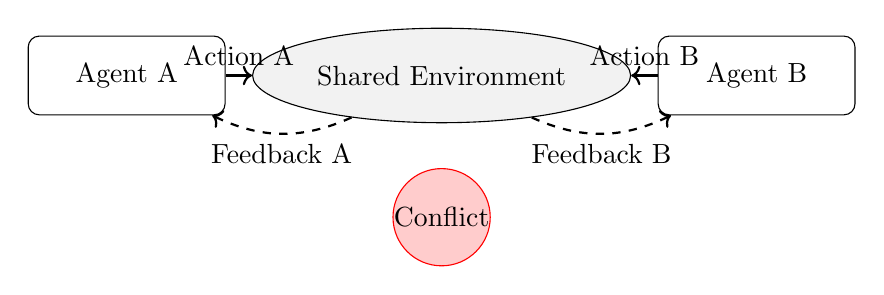
\begin{tikzpicture}[
  agent/.style={rectangle, draw, rounded corners, minimum width=2.5cm, minimum height=1cm, align=center},
  env/.style={ellipse, draw, minimum width=3.5cm, minimum height=1.2cm, align=center, fill=gray!10},
  arrow/.style={->, thick},
  feedback/.style={->, dashed, thick},
  conflict/.style={circle, draw=red, fill=red!20, minimum size=1cm, inner sep=0pt}
]

% Nodes
\node[agent] (A) at (-4, 0) {Agent A};
\node[agent] (B) at (4, 0) {Agent B};
\node[env] (E) at (0, 0) {Shared Environment};

% Arrows from agents to environment
\draw[arrow] (A) -- node[above] {Action A} (E);
\draw[arrow] (B) -- node[above] {Action B} (E);

% Feedback loops
\draw[feedback] (E) to[bend left=25] node[below] {Feedback A} (A);
\draw[feedback] (E) to[bend right=25] node[below] {Feedback B} (B);

% Optional: conflict indicator
\node[conflict] at (0, -1.8) {Conflict};

\end{tikzpicture}
\caption{Generic model of unaware adversaries: agents act on a shared environment, receive feedback only via its state, and have no direct communication or awareness of their mutual antagonism.}
\label{fig:unaware_adversary_loop}
\end{figure}


\section{Case Studies}
\textit{The following models are intentionally simplified to expose coupling structure rather than to serve as predictive simulations}. The mathematics used are illustrative and are not themselves novel analytical formulations deserving of scrutiny.

In two of the Case Studies, we intentionally extend the analysis beyond diagnosis and mitigation to sketch speculative constructions (e.g., the Gradient-Paced BGP Advertiser and the Pedagogical GAN). These are not presented as finished algorithms or protocol proposals, nor as claims of empirical superiority. Rather, they serve a narrower purpose: to demonstrate that the unaware-adversary framework is not merely descriptive, but generative — capable of inspiring non-obvious architectural ideas once a system’s conflict structure is made explicit.

As with the simplified mathematical models used throughout, these constructions should be read as conceptual exemplars, not as validated designs of network protocol algorithms or GAN architecture. Their value lies in showing what kind of ideas fall out of the framework, not in asserting that these particular instantiations are ready for deployment or adoption.

\subsection{Thermostatic Conflict: The Heater-A/C Dyad}
Our canonical example involves a room containing two physically distinct and uncoordinated devices: a radiator governed by a building-level thermostat and a window air-conditioning unit with its own integrated controls. This situation is common in older buildings or offices where supplemental climate control is added. Conflict arises when the setpoints are in opposition; for example, the building heat is set to maintain $22^\circ$C while the window A/C is set by an occupant to cool the room to $20^\circ$C. If the room temperature drifts to $21^\circ$C, both systems will activate, leading to a direct conflict. We can model the temperature dynamics and energy cost as follows:
\begin{align*}
\frac{dT}{dt} &= -k(T - T_{\text{ext}}) + P_H u_H(t) - P_C u_C(t) \\
\text{Cost}~(J) &= \int_{0}^{t_{\text{final}}} \left(C_H u_H(t) + C_C u_C(t)\right)\,dt
\end{align*}

Here, $u(t)$ is the control signal (1 if on, 0 if off) for the heater ($H$) and cooler ($C$), $P_H$ and $P_C$ are their respective thermal powers, and $C_H$ and $C_C$ are their electrical power draw (W). The total energy cost, $J$, in the adversarial configuration is orders of magnitude higher than in a stable configuration, for no improvement in temperature stability.

\subsection{Email Deliverability Conflict (Open-Loop)}
A compelling open-loop example occurs in corporate IT systems. Consider two agents sending email from the same domain (\texttt{@company.com}):
\begin{itemize}
    \item \textbf{Agent A (Marketing Platform):} Its objective is to maximize email sends for a campaign, blasting 500,000 emails in an hour.
    \item \textbf{Agent B (Transactional System):} Its objective is to ensure reliable delivery of critical password reset or receipt emails.
\end{itemize}
The shared environment is the company's domain reputation with email providers (e.g., Google, Microsoft). Agent A's action (the email blast) degrades this reputation, causing Agent B's critical emails to be marked as spam or blocked. The feedback loop is open because the failure of the password reset emails provides no direct signal back to the marketing platform. Agent A's performance metrics are unaffected by the harm caused to Agent B, so it continues its behavior without correction. 

\subsection{Interpretation Failure leading to Auto-scaling conflict}
Consider a microservices architecture where two services independently manage their resource allocation:
\begin{itemize}
\item \textbf{Service A} (API Gateway): Auto-scales based on CPU usage, adding instances when CPU > 80%
\item \textbf{Service B} (Database): Auto-scales based on request queue depth, adding capacity when queue > 100 requests
\end{itemize}
Both services have access to comprehensive metrics dashboards showing:
\begin{itemize}
\item Their own performance metrics
\item Their peer's scaling activities
\item System-wide resource utilization
\item Historical scaling patterns
\end{itemize} 
The information is available, but neither service possesses the logic to recognize that their peer's scaling decision invalidates their own. When Service A scales up due to high CPU, it generates more database requests. Service B observes its queue filling and scales up. The additional database capacity briefly reduces queue depth, which reduces back-pressure on Service A. Service A interprets this as successful load handling and scales up further (or perhaps a more likely configuration would have it do the opposite - scale down as cost savings measure. This distinction should not be important for our point, which is that it creates unintended oscillations.) The cycle repeats, creating cascading over-provisioning.

This exemplifies pure interpretation failure. The feedback loop is closed—both agents receive real-time signals about each other's behavior. But recognizing that "my peer's scaling activity is negating my scaling decision" requires:
\begin{enumerate}
  \item Causal reasoning across service boundaries
  \item Modeling the indirect coupling between CPU load and database queue depth
  \item Maintaining temporal context to detect oscillatory patterns
\end{enumerate}
An individual service's auto-scaling logic is optimized for computational efficiency: a simple threshold-based rule executing in milliseconds. The interpretive burden of higher-order analysis—detecting mutual invalidation across a delayed feedback loop—exceeds its analytical budget.

The solution, per the Observability Principle, is not merely to surface more metrics, but to pre-compute and inject the higher-order signal: a "scaling coordination score" that explicitly flags when peer scaling activities are causally linked. This transforms a complex inference problem into a first-order observable signal.

\subsection{Systemic Opposition in Urban Planning}
Perhaps the most societally significant examples of unaware adversaries occur in socio-technical systems like urban planning. Consider two municipal departments with laudable but conflicting mandates:
\begin{itemize}
    \item \textbf{The Transportation Department:} Tasked with mitigating traffic congestion, its primary Key Performance Indicator (KPI) is maintaining a high Level of Service (LOS) on major arterial roads, a standard defined in the \textit{Highway Capacity Manual} \cite{HCM2022}. A high LOS corresponds to low traffic density and high travel speeds. The department's primary tool is increasing road capacity ($K$) by adding lanes.
    \item \textbf{The Urban Planning Department:} Tasked with addressing housing shortages and promoting sustainability, its goal is to encourage dense, walkable, Transit-Oriented Development (TOD).
\end{itemize}
These two locally-optimized strategies become potent unaware adversaries. The core of the conflict can be formally captured using standard models from transportation engineering. A widely used relationship to model the effect of congestion on travel time is the Bureau of Public Roads (BPR) formula \cite{BPR1964}:

\begin{align*}
t &= t_0 \left[ 1 + \alpha \left( \frac{V_{\text{base}} + \gamma K}{K} \right)^\beta \right] \\
  &= t_0 \left[ 1 + \alpha \left( \frac{V_{\text{base}}}{K} + \gamma \right)^\beta \right]
\end{align*}


Here, $t$ is the actual travel time on a road segment, $t_0$ is the free-flow travel time (with no traffic), $V$ is the traffic volume (vehicles per hour), and $K$ is the practical capacity of the road. The parameters $\alpha$ (typically $\approx 0.15$) and $\beta$ (typically $\approx 4$) determine the severity of congestion effects. The Transportation Department's objective is to minimize $t$ by increasing $K$. Here, $K$ is our capacity expansion proxy, in lane-km.

Concurrently, the Planning Department approves dense residential projects. The immediate effect is an increase in the base number of trips originating in the area, contributing to a higher traffic volume $V$. However, the more insidious coupling occurs through the phenomenon of \textbf{induced demand}. The Transportation Department's expansion of a highway temporarily reduces travel time $t$, making driving faster and more attractive. This, in turn, fuels suburban growth and causes more people to drive, increasing the total traffic volume $V$.

This effect has been empirically verified and is known as the "Fundamental Law of Road Congestion," which states that the total vehicle-kilometers traveled (VKT) in a metropolitan area increases in direct proportion to the available lane-kilometers of roadways \cite{Duranton2011}. We can model this relationship simply as:
\[
V = V_{\text{base}} + \gamma K
\]
where $V_{\text{base}}$ represents the volume from existing development and $\gamma K$ represents the new volume induced by the capacity expansion itself.

The adversarial loop is now clear. Substituting the induced demand model into the BPR formula reveals the systemic trap:
\[
t = t_0 \left[ 1 + \alpha \left( \frac{V_{\text{base}} + \gamma K}{K} \right)^\beta \right] = t_0 \left[ 1 + \alpha \left( \frac{V_{\text{base}}}{K} + \gamma \right)^\beta \right]
\]
When the Transportation Department increases capacity ($K$), the term $\frac{V_{\text{base}}}{K}$ decreases, which is the intended effect of alleviating existing congestion. However, the presence of the induced demand constant $\gamma$ means that as $K$ becomes very large, the ratio inside the parentheses does not approach zero, but rather approaches $\gamma$. The travel time $t$ does not return to the free-flow time $t_0$, but instead approaches a new, congested equilibrium:
$$
t \to t_0 \left( 1 + \alpha \gamma^\beta \right) \quad \text{as } K \to \infty
$$

\begin{itemize}
\item \textit{Since $\gamma$ represents the induced demand coefficient, if $\gamma \approx 1$ (as suggested by the "Fundamental Law of Road Congestion") , the equilibrium travel time remains significantly higher than free-flow.}
\end{itemize}

Each department successfully meets its own local KPIs—lanes are built, and housing is approved—yet the system as a whole suffers from persistent congestion despite massive capital expenditure. The agents are locked in a state of policy-induced homeostasis, where each one's logical, well-intentioned actions systemically negate the efforts of the other.

This represents not only misaligned incentives, but also a limited optimization scope. We can add a formal constraint as we defined Bounded Processing Capacity in our framework, to call out the problem:

Let $A = \{a_1, a_2, \dots, a_n\}$ be the set of all relevant state variables. Formally, each department optimizes over a strict subset of the relevant state variables; induced-demand dynamics fall outside both objective scopes

By the Bounded Processing Capacity defined in Section 3, we should ensure each agent has an appropriate Attention Budget so that Induced Demand and VKT have bandwidth to process these information signals.

\begin{itemize}
    \item \textbf{Transportation Dept:} optimizes over $\{\text{LOS, capacity } K\}$
    \item \textbf{Planning Dept:} optimizes over $\{\text{housing units, density}\}$
    \item \textbf{Neither:} optimizes over $\{\text{induced demand } \gamma, \text{long-term VKT}\}$
\end{itemize}

\subsection{Interdomain Routing Instability and the YouTube/Pakistan BGP Hijack}

The dynamic of independent agents pursuing local optimizations at the expense of global system health extends from urban planning to the core architecture of the internet itself. The Border Gateway Protocol (BGP) \cite{rfc4271} governs interdomain routing across the Internet, enabling thousands of autonomous systems (ASes) to exchange reachability information. While BGP is highly flexible, its decentralized and policy-driven design creates opportunities for emergent instability. This subsection presents a general case of unaware adversarial interaction in interdomain traffic engineering, followed by a concrete, high-impact example: the 2008 YouTube/Pakistan BGP hijack incident.

\subsubsection*{General Case: Unaware Traffic Engineering Between ASes}

Consider two neighboring ASes:

\begin{itemize}
    \item \textbf{AS A (Transit Provider):} Uses internal link metrics and MEDs \cite{rfc4451} to load-balance traffic and minimize internal congestion.
    \item \textbf{AS B (Content Provider):} Optimizes for inbound performance by modifying BGP community tags and selectively announcing prefixes.
\end{itemize}

Both systems reactively adjust (typically via some mechanism outside of BGP itself) \cite{draft-idr-pr-04} their routing announcements based on local utility functions—CPU load, latency, throughput—but do so without coordination. Their interaction takes place through BGP advertisements and path selection behavior, producing a shared environment susceptible to instability.

Each AS modulates its route announcements as a function of observed performance:

\[
R_A(t + \Delta t) = f_A(R_B(t), L_A(t)) \quad\text{and}\quad R_B(t + \Delta t) = f_B(R_A(t), L_B(t))
\]

This coupling forms a delayed feedback loop. The system may enter oscillatory regimes or route flap storms, degrading routing stability and increasing global convergence latency \cite{labovitz1997}.

\paragraph{Proposed Mitigation: Gradient-Paced BGP Advertiser (GPBA)}

Here, we demonstrate the framework’s usefulness by sketching a hypothetical mitigation strategy for interdomain routing: the \textbf{Gradient-Paced BGP Advertiser (GPBA)}. Rather than impose fixed rate limits, GPBA adapts the pace of route advertisement based on the environmental sensitivity observed at the peer:

\[
\Delta t_{\text{propagation}} \propto \left\| \frac{dR_{\text{remote}}}{dR_{\text{local}}} \right\|
\]

This principle discourages volatile updates by throttling agents whose announcements produce outsized ripples in routing state. Unlike traditional filters, GPBA uses a reflexive meta-policy: it applies only when sensitivity is high and relaxes when peers demonstrate robustness or stability. This maintains responsiveness while discouraging feedback-amplifying behavior.

\subsubsection*{Case Study: The YouTube/Pakistan Hijack (2008)}

In February 2008, Pakistan Telecom (AS17557) attempted to implement a government-ordered block of YouTube by announcing a more-specific prefix (208.65.153.0/24) intended for internal blackholing. This announcement was mistakenly propagated to PCCW (AS3491), a major transit provider, which further distributed the route across the global Internet.

Due to BGP’s path selection rules, the hijacked prefix—which was more specific than YouTube’s legitimate announcement—was globally preferred, redirecting worldwide traffic to a null route in Pakistan. YouTube was rendered inaccessible for several hours \cite{cowie2008}.

This incident demonstrates classic unaware adversarial dynamics:
\begin{itemize}
    \item \textbf{Independent Objectives:} Pakistan Telecom sought national censorship; PCCW aimed to maintain routing continuity and performance.
    \item \textbf{Shared Environment:} The global BGP routing table.
    \item \textbf{Indirect Coupling:} PCCW’s propagation choices were influenced by AS17557’s unexpected prefix origin.
    \item \textbf{Antagonistic Effect:} Global denial of service for YouTube, triggered by local policy and lack of propagation checks.
\end{itemize}

\paragraph{Could GPBA Have Mitigated This?}

A GPBA-aware edge at PCCW could have detected that:
\begin{enumerate}
    \item The origin of 208.65.153.0/24 (AS17557) was highly anomalous.
    \item The route produced a high volatility score in terms of downstream reachability change.
\end{enumerate}

Rather than immediately propagate the route, the GPBA heuristic would have increased the propagation delay or required additional validation. This passive reflexivity—without requiring global RPKI \cite{rfc8210}  or semantic understanding of the policy intent—could have bought time for human intervention or for automated anomaly detectors to act.


\paragraph{General Insight}

The YouTube/Pakistan incident underscores the vulnerability of loosely coordinated protocols like BGP to unaware adversarial dynamics. GPBA-style mechanisms offer a path forward by embedding environmental reflexivity into protocol behavior. Rather than controlling agent behavior through centralized rules, GPBA designs the feedback surface itself to discourage destabilizing actions.  In the language of our design principles, it represents a sophisticated form of the Observability Principle, where the system observes its own sensitivity to change and creates feedback to regulate it.


\subsection{From Designed Conflict to a Novel Research Hypothesis: The Pedagogical GAN}
The standard Generative Adversarial Network (GAN) \cite{Goodfellow2014} provides a powerful case study for our framework. It is a system of two agents, a Generator ($G$) and a Discriminator ($D$), locked in a designed, zero-sum game. This adversarial dynamic, however, is notoriously unstable and suffers from practical issues like vanishing gradients, where $D$ becomes too proficient, leaving $G$ with no learning signal. The original authors' first solution was the heuristic "non-saturating" loss, an immediate modification that sought a stronger, more reliable gradient for $G$. This established the central challenge in the field: managing the adversarial dynamic for stable and efficient training.

In the years since, the dominant paradigm for GAN stabilization has become one of \textbf{gradient control}. Landmark models like Wasserstein GAN (WGAN) \cite{Arjovsky2017} and its successor WGAN-GP \cite{Gulrajani2017} diagnosed the problem as being rooted in the geometry of the loss landscape. Their solution, which now represents the state-of-the-art, is to \textit{tame and constrain} the discriminator's function (e.g., by enforcing a Lipschitz condition) to guarantee that it always provides a smooth and informative gradient to the generator. This philosophy is about preventing conflict from becoming destructive by carefully limiting the power of the adversary.

Our framework of unaware adversaries prompts a different line of inquiry. Instead of asking, "How do we control the conflict?", we ask, "Can we redesign the agents' objectives to make the conflict more productive?" This leads us to sketch a perhaps novel approach that stands in philosophical opposition to gradient control. We term this the \textbf{Pedagogical GAN} here.

The core idea of the Pedagogical GAN is to change the generator's objective from simply fooling the discriminator to actively teaching it as efficiently as possible. We formalize this by proposing that the generator should seek to \textit{maximize} the discriminator's learning signal. The generator's objective function becomes:
$$ \max_{G} \left\| \nabla_{D} \mathcal{L}(D, G) \right\|_2 $$
Here, $\mathcal{L} (D, G)$ is the standard discriminator loss. The generator is now explicitly incentivized to find samples that lie on the steepest parts of the discriminator's loss landscape. It becomes a "Socratic tutor" that seeks to \textit{weaponize} the gradient for accelerated learning, not suppress it.

This approach represents a conceptual departure from gradient-control-based stabilization. It is distinct from other cooperative frameworks, like Cooperative Teacher or Feature Map Distillation \cite{hu2022discriminatorcooperatedfeaturemapdistillation} and  Unrolled GANs \cite{Metz2016}, which use strategic foresight, or other non-antagonistic models that alter loss functions to escape the zero-sum game \cite{Xie2016}. Instead, it can be viewed as the principled and extreme conclusion of the line of thinking that began with the very first non-saturating GAN loss. We have not found this exact objective stated explicitly elsewhere; regardless, we only use it here as a conceptual exemplar of framework-driven ideation. 


\section{A Taxonomy of Unaware Adversarial Systems}
To demonstrate the analytical power of this framework, we now apply the taxonomy to our diverse case studies. As shown in Table \ref{tab:taxonomy_analysis}, this classification not only organizes the examples but also reveals critical insights into the underlying dynamics of each type of conflict and prescribes a UA Principle for mitigation strategy.

\begin{table}[h!]
  \caption{Taxonomy Analysis of Case Studies}
  \label{tab:taxonomy_analysis}
  \centering
  \begin{tabular}{lllllll}
    \toprule
    \textbf{Case} & \textbf{Domain} & \textbf{Coupling} & \textbf{Feedback} & \textbf{Complexity} & \textbf{Symmetry} & \textbf{Principle} \\
    \midrule
    4.1 & Mechanical & Physical & Closed-Loop & First-order & Symmetric & Hierarchy \\
    4.2 & Digital & Informational & Open-Loop & Higher-order & Asymmetric & Observability \\
    4.3 & Digital & Informational & Closed-Loop & Higher-order & Symmetric & Observability \\
    4.4 & Social & Environmental & Closed-Loop &  Multi-order & Asymmetric & Incentive \\
    4.5 & Net Infra. & Informational & Semi-Open & Higher-order & Asymmetric & Observability \\
    4.6 & Digital & Informational & Closed-Loop & Higher-order & Asymmetric & Incentive \\   
    \bottomrule
  \end{tabular}
\end{table}

The taxonomy reveals a critical distinction: in the open-loop conflict, the harm is asymmetric and the adversarial agent receives no corrective feedback, suggesting such problems can persist undetected for long periods. This contrasts with the noisy, symmetric inefficiency of the closed-loop thermostat conflict.

The BGP case introduces a "semi-open-loop," where an agent receives operational feedback that its actions have propagated (the route was accepted) but remains blind to the wider, negative systemic consequences of that action (the denial of service).

\section{Implications for System Design: From Mitigation to Architecture}

An understanding of unaware adversaries does more than explain a class of failures; it provides a powerful set of principles for designing robust, efficient, and intelligent systems. By consciously analyzing the potential for emergent conflict, designers can move from a reactive posture of debugging and mitigation to a proactive one of thoughtful system architecture. The framework allows us to ask critical questions at the design stage: Who are the agents in this system? What environment do they share? How are they coupled? And most importantly, how could their local objectives lead to global conflict? The answers lead to a set of clear design principles.

\subsection{The Observability Principle}   
\begin{itemize}
\item{Make System-Wide Effects Locally Apparent}
\item{\textbf{AND} provide signals in a form that matches the agent's processing capacity}
\item{\textbf{AND} explicitly surface higher-order implications that agents might not compute themselves}
\end{itemize}
This principle directly targets the most insidious conflicts: the open-loop, asymmetric cases where one agent operates completely unaware of the harm it causes. The solution is to create a feedback channel where one does not naturally exist.

\begin{description}
    \item[The Problem:] As seen in the Email Deliverability case, the marketing platform's performance metrics (e.g., emails sent) are decoupled from the negative externality it creates (degraded domain reputation). The agent is flying blind to the true system-wide cost of its actions.
    \item[The Design Solution:] Instrument the system to make the shared state visible and, crucially, to integrate that state into each agent's local decision-making context. Don't just provide the marketing team with a dashboard showing their send volume; create a shared, top-level "Domain Health" or "Deliverability Score" that is a KPI for \textit{both} the marketing team and the IT department. When the marketing platform initiates a blast, it should see a real-time dip in a metric it is also responsible for. This makes the invisible visible and forces the unaware adversary to reckon with the consequences of its behavior.
\end{description}

\subsection{The Incentive Principle: Redefine "Winning" to Induce Cooperation}
For conflicts where agents have fundamentally misaligned goals, imposing external controls can be brittle and inefficient. A more elegant and robust solution is to redesign the agents' objective functions so that cooperation becomes an emergent property of them pursuing their own, revised goals.

\begin{description}
    \item[The Problem:] In the Urban Planning and standard GAN examples, each agent "winning" by its local definition leads to collective failure (gridlock) or instability (vanishing gradients). Their objectives are locked in zero-sum or mutually destructive patterns.
    \item[The Design Solution:] This is the most transformative principle. Instead of just adding a coordinating layer, change what it means for an agent to succeed. Our proposal for the \textbf{Pedagogical GAN} is the canonical example: we shift the Generator's objective from "fool the Discriminator" to "maximize the Discriminator's learning rate." This reframes the adversary not as an opponent to be defeated, but as a student to be taught efficiently. In the Urban Planning context, it would mean replacing department-level KPIs like "Level of Service" and "Housing Units Approved" with a single, shared, system-level objective, such as "Minimize average citizen commute time" or "Maximize accessibility score." This forces the departments to find a cooperative, globally optimal solution.
\end{description}

\subsection{The Hierarchy Principle: Appoint a Single Arbiter for Contested States}
When agent objectives are simple, directly oppositional, and tightly coupled through a physical state, the most effective solution is often to remove autonomy and establish a clear control hierarchy.

\begin{description}
    \item[The Problem:] The Heater-A/C dyad is a perfect example. Two simple agents are fighting a direct, symmetric battle over a single, continuous variable: room temperature. Their control logic is too simple to negotiate a truce.
    \item[The Design Solution:] Institute a higher-level arbiter or a "master controller" that has authority over both agents and manages the contested resource. The solution is a single, smart thermostat that controls both the heat and the A/C. It becomes the sole source of truth for the room's temperature and can make intelligent decisions (e.g., defining a deadband between heating and cooling setpoints) that are impossible for the independent agents. This principle applies to any system fighting over a fungible resource, from CPU cycles in a computer to water rights in a river basin.
\end{description}

By applying these principles, the framework of unaware adversaries becomes a generative tool. It equips a designer to anticipate failure modes and architect systems that are not only resilient to conflict but are designed from the ground up for emergent cooperation.

\section{Discussion}
\subsection{The Architecture of Interaction}
The primary contribution of this paper is a framework that serves not only as a descriptive and diagnostic tool but as a generative engine for system design. We demonstrated this generative capacity twice over, deriving novel solution ideas in two disparate domains: the \textbf{Pedagogical GAN} for machine learning and the \textbf{Gradient-Paced BGP Advertiser (GPBA)} for network protocol design. Both concepts emerged directly from applying our framework's lens to a well-known problem. In each case, instead of accepting the standard adversarial dynamic as given, the framework prompted a fundamental question: "How can we redesign the agent's interaction rules to make the conflict less destructive or even productive?" The proposed solutions—one that reframes training as teaching, the other that paces communication based on systemic sensitivity—are deliberate architectural choices about the nature of the agents' interaction. They represent a significant philosophical departure from conventional approaches that focus on adversarial suppression or fixed rate-limiting.

While the Pedagogical GAN proposal would require empirical validation to prove its worth, that is not the point of its inclusion; its conceptual origin is provided as evidence of the framework's creative value. It is the direct result of applying the \textbf{Incentive Principle}, one of the three core design strategies that emerge from our analysis. The other principles are equally direct consequences of the framework. The \textbf{Observability Principle} is the clear solution to the open-loop, asymmetric harm seen in the Email Deliverability case, while the \textbf{Hierarchy Principle} is the obvious remedy for the simple, symmetric conflict of the Heater-A/C dyad. The framework, therefore, does not just identify problems; it naturally leads to a specific class of solutions tailored to the type of conflict.

The concept of unaware adversaries is especially salient today. As we continue to build ever more complex, decentralized systems—from microservice architectures and the Internet of Things to multi-agent AI ecosystems and smart cities—the potential for emergent, unintended conflict grows exponentially. Our traditional engineering and debugging practices, which focus on verifying the correctness of individual components, are insufficient for addressing failures that arise from the negative space \textit{between} those components. The problem is not that the transportation department's models are wrong or that the marketing platform's code has a bug; the problem is that the system's architecture creates incentives for globally destructive, locally optimal behavior.

Ultimately, this framework encourages a crucial shift in perspective for architects and designers. It moves the focus from the design of agents in isolation to the design of the environment they share and the incentive landscape they inhabit. By analyzing the structure of the coupling and the nature of the feedback loops, we can stop being surprised by "policy resistance" or "unintended consequences" and start architecting systems where cooperation is not an afterthought, but an emergent property of the system's fundamental design.

\subsection{Relation to Classical Control Theory}
Many of the systems described in our case studies (oscillating on/off controllers, pathological GAN dynamics, BGP route convergence) are familiar terrain in classical control theory. Such systems can often be modeled as composite dynamical systems and analyzed using tools like Lyapunov stability, observability, and controllability \cite{Khalil2002}.

A compelling example of this distinction comes from classical PID control. The P, I, and D terms can be viewed as three "unaware adversaries" - independent control laws with different temporal objectives (present error, accumulated error, rate of change) simultaneously acting on a shared output. (This is an analogy rather than a literal agent decomposition; the value is in highlighting architectural coupling, not intentional autonomy. Unlike the other case studies, PID terms are intentionally designed to counterbalance each other—their interaction is coordinated by design, even if we can analyze them through an unaware-adversary lens.) While stability analysis tells us under what conditions this composite system converges, our framework asks: what if the P term's aggressive response triggers instability in the D term's derivative estimate? This is not a question of mathematical stability but of architectural choice about how to structure agent interactions.

Another distinction from this formal standpoint, is that while the existence (or absence) of a global Lyapunov function may determine whether the system exhibits convergence to equilibrium, our framework highlights that stability alone is not the only goal. \textit{A system can be stable and still fail}. Many real-world adversarial pathologies - such as traffic congestion equilibria \cite{Downs1992}, or GANs collapsing to degenerate outputs \cite{Goodfellow2014, Arjovsky2017} - are cases where systems settle into \textit{undesirable equilibria, not chaotic instability}.

Framing these as systems of "unaware adversaries" surfaces a complementary perspective that classical tools, by design, abstract away: that each agent is acting rationally within its own feedback loop, but their combined behavior produces outcomes no one intended and no one benefits from. This is not merely a problem of instability; it is rather a problem of emergent misalignment.

What our framework offers is not a substitute for classical  analysis, but a formalized way to highlight systems that look stable on paper but can exhibit pathological behavior due to unrecognized structural conflicts between agents. Classical control theory excels when systems can be modeled from first principles and the question is convergence, stability margins, or optimal control law design. 
The Unaware Adversaries framework is most valuable when: 
\begin{enumerate}
\item{the system is too complex for tractable first-principles modeling (e.g., organizational dynamics, multi-stakeholder systems),}
\item{the agents themselves are designed/intelligent entities with goals (not just passive dynamics), or}
\item{the pathology lies in emergent misalignment between rational actors rather than parametric instability.}
\end{enumerate}

The frameworks are thus complementary - classical theory for well-defined dynamical systems, unaware adversaries for socio-technical systems where intentionality matters.

For example, the Pedagogical GAN proposed earlier does not reject the gradient-based framing of GAN dynamics. Instead, it reframes the design question: what if we architected the generator and discriminator not as antagonists, but as collaborators with asymmetric knowledge? This reframing doesn’t negate formal stability concerns, it simply shifts attention toward the shape and utility of the learning signal, and not solely its convergence properties.

While the framework's Observability Principle emphasizes making system-wide effects visible, visibility alone is insufficient when agents lack the processing capacity to interpret complex or higher-order signals.
Consider the Email Deliverability case: the marketing platform could theoretically monitor global SMTP rejection rates, DNS blacklist statuses, and reputation scores. But recognizing that their blast is the cause of degraded reputation requires: 
\begin{enumerate}
\item{temporal correlation analysis,} 
\item{understanding of cumulative effects, and}
\item{attribution across delayed feedback.}
\end{enumerate}
This interpretive burden may exceed the agent's analytical budget.
Effective mitigation strategies must account not only for what information agents can access, but what information they can process and act upon given their bounded rationality. Signals must be pre-processed, aggregated, or simplified to match agent capabilities—or alternatively, agents must be equipped with sufficient analytical resources to extract meaning from raw environmental data

The tools of nonlinear systems theory - comprehensively covered in foundational texts such as Khalil's Nonlinear Systems  \cite{Khalil2002} - provide the rigorous formalisms for system stability and convergence. When such modeling is tractable, these methods should be the first line of analysis.  But when full modeling is infeasible, or when coordination failure arises from structural blindness rather than stochastic noise, our lens provides a complementary mode of reasoning that emphasizes intentionality, partial observability, and emergent conflict.

If classical control tells us whether a system will converge, the framework of unaware adversaries helps us ask: to what, and why?


\section{Directions for Future Research}
This framework opens several avenues for future inquiry, most notably:
\begin{itemize}
    \item The formal implementation and empirical validation of the proposed \textbf{Pedagogical GAN}. This would involve developing the necessary regularization techniques to stabilize the training dynamic and testing its performance against baseline models and gradient control methods like WGAN-GP.
    \item Analysis of unaware conflict in large-scale distributed AI systems, such as competing recommendation algorithms on a single platform.
    \item Application of the unaware adversary lens to AI alignment and interpretability, especially in ensembles of independently trained agents.
    \item The formal specification and empirical validation of the proposed \textbf{Gradient-Paced BGP Advertiser (GPBA)}. This would involve simulation in environments like BGPStream to test its efficacy in dampening route flaps and mitigating the propagation speed of malicious hijacks compared to existing mechanisms like route flap damping.

\end{itemize}

\section{Conclusion}
The concept of unaware adversaries provides a valuable lens for analyzing and resolving a significant class of system failures. By moving beyond debugging individual components to architecting the environment in which they interact, we can mitigate and even prevent emergent, destructive conflict. This paper defined a formal framework for this analysis and demonstrated its utility across mechanical, digital, and socio-technical systems. Crucially, we have shown this framework to be more than just descriptive; it is a generative tool for innovation. The derivation of two distinct and plausible solutions, the Pedagogical GAN and the Gradient-Paced BGP Advertiser, proves that a principled understanding of emergent conflict can inspire novel designs for more robust, stable, and cooperative systems.

\section*{Acknowledgments}
The author acknowledges and appreciates the feedback received on /r/ControlTheory and HackerNews. The paper is stronger because of kind strangers /u/NaturesBlunder and troelsSteegin@HN who questioned or commented on my paper's first draft.

\begin{thebibliography}{99}

\bibitem{Senge1990}
Peter M. Senge.
\newblock \textit{The Fifth Discipline: The Art \& Practice of The Learning Organization}.
\newblock Doubleday, 1990.

\bibitem{Goodfellow2014}
Ian J. Goodfellow, Jean Pouget-Abadie, Mehdi Mirza, Bing Xu, David Warde-Farley, Sherjil Ozair, Aaron Courville, and Yoshua Bengio.
\newblock Generative Adversarial Networks.
\newblock In \textit{Advances in Neural Information Processing Systems 27}, pages 2672--2680, 2014.

\bibitem{Arjovsky2017}
Martin Arjovsky, Soumith Chintala, and Léon Bottou.
\newblock Wasserstein GAN.
\newblock \textit{arXiv preprint arXiv:1701.07875}, 2017.

\bibitem{Gulrajani2017}
Ishan Gulrajani, Faruk Ahmed, Martin Arjovsky, Vincent Dumoulin, and Aaron Courville.
\newblock Improved Training of Wasserstein GANs.
\newblock In \textit{Advances in Neural Information Processing Systems 30}, pages 5767--5777, 2017.

\bibitem{Metz2016}
Luke Metz, Ben Poole, David Pfau, and Jascha Sohl-Dickstein.
\newblock Unrolled generative adversarial networks.
\newblock \textit{arXiv preprint arXiv:1611.02163}, 2016.

\bibitem{Xie2016}
Jianwen Xie, Yang Lu, Song-Chun Zhu, and Ying Nian Wu.
\newblock Cooperative Training of Descriptor and Generator Networks.
\newblock \textit{arXiv preprint arXiv:1609.09408}, 2016.

\bibitem{Downs1992}
Anthony Downs.
\newblock \textit{Stuck in Traffic: Coping with Peak-Hour Traffic Congestion}.
\newblock Brookings Institution Press, 1992.

\bibitem{HCM2022}
Transportation Research Board.
\newblock \textit{Highway Capacity Manual, 7th Edition: A Guide for Multimodal Mobility Analysis}.
\newblock National Academies of Sciences, Engineering, and Medicine, 2022.

\bibitem{BPR1964}
Bureau of Public Roads.
\newblock \textit{Traffic Assignment Manual}.
\newblock U.S. Department of Commerce, Urban Planning Division, 1964.

\bibitem{Duranton2011}
Gilles Duranton and Matthew A. Turner.
\newblock The Fundamental Law of Road Congestion: Evidence from US Cities.
\newblock \textit{American Economic Review}, 101(6): 2616--52, 2011.

\bibitem{labovitz1997}
Craig Labovitz, Abha Ahuja, Abhijit Bose, and Farnam Jahanian.
\newblock Delayed Internet Routing Convergence.
\newblock In \textit{Proceedings of ACM SIGCOMM}, 1997.

\bibitem{cowie2008}
Jim Cowie.
\newblock \textit{Pakistan Hijacks YouTube}.
\newblock Renesys Blog, February 24, 2008.
\newblock Available at: \url{https://web.archive.org/web/20210506213233/https://www.renesys.com/2008/02/pakistan-hijacks-youtube-1/} (archived from the original).

\bibitem{rfc4271}
Y. Rekhter, T. Li, and S. Hares, editors.
\newblock \textit{A Border Gateway Protocol 4 (BGP-4)}.
\newblock Request for Comments 4271, Internet Engineering Task Force, January 2006.
\newblock \url{https://datatracker.ietf.org/doc/html/rfc4271}.

\bibitem{rfc4451}
D. McPherson, V Gill, editors.
\newblock \textit{BGP MULTI\_EXIT\_DISC (MED) Considerations}.
\newblock Request for Comments 4451, Internet Engineering Task Force, March 2006.
\newblock \url{https://datatracker.ietf.org/doc/html/rfc4451}

\bibitem{rfc8210}
R. Bush, R. Austein, editors.
\newblock \textit{The Resource Public Key Infrastructure (RPKI) to Router Protocol, Version 1}
\newblock Request for Comments: 8210, Internet Engineering Task Force (IETF), September 2017.
\newblock \url{https://datatracker.ietf.org/doc/html/rfc8210}

\bibitem{draft-idr-pr-04}
X. Xu, S. Hegde, K. Talaulikar, M. Boucadair, C. Jacquenet, editors.
\newblock \textit{ Performance-based BGP Routing Mechanism draft-ietf-idr-performance-routing-04}
\newblock Internet-Draft, Internet Engineering Task Force (IETF), August 2024.
\newblock \url{https://www.ietf.org/archive/id/draft-ietf-idr-performance-routing-04.txt}

\bibitem{Khalil2002}
Hassan K. Khalil.
\newblock \textit{Nonlinear Systems, 3rd ed.}
\newblock Prentice Hall 2002

\bibitem{hsu-lyapunov}
Hsu, Jules C.
\newblock \textit{Control Systems: An Introduction with MATLAB}
\newblock McGraw-Hill, 1998.

\bibitem{hu2022discriminatorcooperatedfeaturemapdistillation}
Tie Hu and Mingbao Lin and Lizhou You and Fei Chao and Rongrong Ji.
\newblock \textit{Discriminator-Cooperated Feature Map Distillation for GAN Compression}
\newblock arXiv 2212.14169.
\url{https://arxiv.org/abs/2212.14169} 

\bibitem{K_factor}
\newblock K Factor (traffic engineering).
\newblock \url{https://en.wikipedia.org/wiki/K_factor_(traffic_engineering)#:~:text=The%20calculation%20for%20the%20K,when%20calculating%20the%20K%20factor.}

\end{thebibliography}

\end{document}
